%%%%%%%%%%%%%%%%%%%%%%%%%%%%%%%%%%%%%%%%%%%%%%%%%%%%%%%%%%%%%%%%%%%%%%%%%%%%%%%%
%2345678901234567890123456789012345678901234567890123456789012345678901234567890
%        1         2         3         4         5         6         7         8
\documentclass[letterpaper, 10 pt, conference]{ieeeconf}  % Comment this line out
                                                          % if you need a4paper
%\documentclass[a4paper, 10pt, conference]{ieeeconf}      % Use this line for a4

\usepackage{float}
                                                          % paper
% uso paquete bookmark para tener bien los outlines.
\usepackage{bookmark}

% Configuro el idioma.
\usepackage[utf8]{inputenc} % Importante para mantener acentos.
\usepackage[spanish, activeacute]{babel} % Requiere: texlive-lang-spanish. Por primera vez hay que ejecutar: texconfig init> log

% Paquete para poder usar acentos en $$.
\usepackage{mathtools}
%\setmathfont{XITS math}

% Para los diagramas de flujo
\usepackage{tikz}
\usetikzlibrary{shapes.geometric, arrows}

% Elementos del diagrama
\tikzstyle{startstop} = [rectangle, rounded corners, 
minimum width=6em, 
minimum height=2em,
text centered, 
draw=black, 
fill=red!30]

\tikzstyle{io} = [trapezium, 
trapezium stretches=true, % A later addition
trapezium left angle=70, 
trapezium right angle=110, 
minimum width=6em, 
minimum height=2em, text centered, 
draw=black, fill=blue!30]

\tikzstyle{block} = [rectangle, 
minimum width=8em, 
minimum height=3em, 
text centered, 
text width=7.5em, 
draw=black, 
fill=white!30]

\tikzstyle{def} = [rectangle, 
minimum width=14em, 
minimum height=3em, 
text centered, 
text width=12em, 
draw=black, 
fill=purple!30]

\tikzstyle{swap_proccess} = [rectangle, 
minimum width=8em, 
minimum height=2em, 
text centered, 
text width=8em, 
draw=black, 
fill=orange!30]

\tikzstyle{process} = [rectangle, 
minimum width=6em, 
minimum height=2em, 
text centered, 
text width=6em, 
draw=black, 
fill=orange!30]

\tikzstyle{decision} = [diamond, 
minimum width=6em, 
minimum height=6em, 
text centered, 
draw=black, 
fill=green!30]
\tikzstyle{arrow} = [thick,->,>=stealth]

\usepackage{siunitx}

% package to get \url
\usepackage{hyperref}
\hypersetup{
  colorlinks=true,
  linkcolor=magenta,
  filecolor=magenta,
  citecolor=magenta,      
  urlcolor=magenta,
}

% Graficos electrónicos
\usepackage{circuitikz}

\IEEEoverridecommandlockouts                              % This command is only
                                                          % needed if you want to
                                                          % use the \thanks command
\overrideIEEEmargins
% See the \addtolength command later in the file to balance the column lengths
% on the last page of the document

\usepackage{graphicx}
\usepackage{graphics}

% styling for matlab/octave code.
\usepackage{matlab-prettifier}
% Configuracion, con esto puede agregar ñ.
\lstset{
  literate={ñ}{{\~n}}1
}

\usepackage{listings}

% The following packages can be found on http:\\www.ctan.org
%\usepackage{graphics} % for pdf, bitmapped graphics files
%\usepackage{epsfig} % for postscript graphics files
%\usepackage{mathptmx} % assumes new font selection scheme installed
%\usepackage{times} % assumes new font selection scheme installed
\usepackage{amsmath} % assumes amsmath package installed
%\usepackage{amssymb}  % assumes amsmath package installed

\title{\LARGE \bf Integrador TP N° 2}

\author{
  Tom\'as Vidal\\
  {\it Arquitectura de Computadoras}\\
  {\it Facultad de Ingenier\'ia, UNLP, La Plata, Argentina.}\\
  {\it 22 de Junio, 2024.}
}                                            % <-this % stops a space


% comienzo

% INTRO


% Figura
\newcommand{\image}[2] {
  \begin{figure}[H]
    \centering
    \includegraphics[width=0.43\textwidth]{./#1.png}
    \caption{#2}
    \label{fig:#1}
  \end{figure}
}

% Codigo
% \begin{lstlisting}[style=Matlab-editor]
% % el código va aca
% dispc("HELLO WORLD");
% \end{lstlisting}

\begin{document}
\maketitle
\thispagestyle{empty}
\pagestyle{empty}

\section{AVR y MARIE}
Para resolver el problema Integrador 2 se empleó nuevamente el algoritmo de ordenamiento Bubble Sort (fig \ref{diag:flujo_bubble_sort}) realizado en Marie previamente, a diferencia de MARIE la arquitectura AVR posee múltiples registros por lo que la implementación del algoritmo fue más fácil en lineas generales. Se emplearon un total de 7 registros, 1 que almacena el cero para hacer operaciones con carry (\textit{ZERO}), uno temporal (\textit{TEMP}), uno para el dato actual del vector \textbf{a[j]} (\textit{currVal}), otro para el siguiente dato \textbf{a[j+1]} (\textit{nextVal}), I y J que son los contadores del \textit{Bubble Sort} y por último \textit{Counter} que es el contador del para hacer mediciones del promedio temporal. No es necesario emplear tanta cantidad de registros, la cantidad de podría minimizar, pero por cuestiones de legilibilidad, \textit{debugeo} (más fácil aislar partes de código, y funciones) y, porque el problema no lo requiere, se hace uso de estos registros. 

\begin{figure}[htbp]
  \footnotesize
  % \centering
  \begin{tikzpicture}[node distance=1.1cm]

    \node (start) [startstop] {Comienzo};
    \node (initcond) [def, below of=start] {a = $<a_0, a_1, \dots, a_n>$};
    \node (def_i_j) [def, below of=initcond] {i=0; j=0};

    \node (i_less_n) [decision, below of=def_i_j, yshift=-0.5cm] {$i<n$};
    \node (print_arr) [process, right of=i_less_n, xshift=2.75cm] {Imprimir arreglo};
    \node (end) [startstop, below of=print_arr, yshift=-0.25cm] {Terminar};

    \node (j_less_n) [decision, below of=i_less_n, yshift=-1.5cm] {$j<n-i-1$};
    \node (inc_i) [process, left of=j_less_n, xshift=-1.4cm, yshift=1.75cm] {$i = i+1$};

    \node (a_gtr_a1) [decision, below of=j_less_n, yshift=-1.75cm] {$a[j]>a[j+1]$};
    \node (inc_j) [process, right of=a_gtr_a1, xshift=1.5cm] {$j = j+1$};

    \node (swap) [swap_proccess, below of=a_gtr_a1, yshift=-1cm] {permutar $ a[j] \leftrightarrow a[j+1]$};

    \draw [arrow] (start) -- (initcond);
    \draw [arrow] (initcond) -- (def_i_j);
    \draw [arrow] (def_i_j) -- (i_less_n);
    \draw [arrow] (i_less_n) -- node[anchor=south] {no} (print_arr);
    \draw [arrow] (print_arr) -- (end);
    \draw [arrow] (i_less_n) -- node[anchor=west] {si} (j_less_n);
    \draw [arrow] (j_less_n) -| node[anchor=south, xshift=1cm] {no} (inc_i);
    \draw [arrow] (j_less_n) -- node[anchor=west] {si} (a_gtr_a1);
    \draw [arrow] (inc_i.north) |- (i_less_n.west);
    \draw [arrow] (a_gtr_a1) -- node[anchor=west] {si} (swap);
    \draw [arrow] (a_gtr_a1) -- node[anchor=south] {no} (inc_j);
    \draw [arrow] (swap) -| (inc_j);
    \draw [arrow] (inc_j.north) |- (j_less_n.north);

  \end{tikzpicture}
  \caption{Diagrama de flujo de Bubble Sort}
  \label{diag:flujo_bubble_sort}
\end{figure}

\section{El código}
Consiste básicamente en 3 partes o funciones: TIME\_AVG\_BUBBLE\_SORT, LOAD\_RND\_VECTOR y BUBBLE\_SORT. Al principio del código se encuentran las definiciones de los registros empleados y las constantes usadas a lo largo de todo el código. Posteriormente se encuentras varios MACROS que facilitan la legilibilidad y la reusablidad de código. Luego viene una sección denominada SETUP que consiste del código que sólo se ejecuta una vez antes del \textit{loop principal}; luego está este \textit{loop}, que no contiene nada ya que no hay que procesar nada continuamente. Y por útlimo esta la sección donde se declaran todas las funciones (son rutinas que guardan los datos previos en el Stack Pointer para poder volver al contexto previo con la instrucción ret), allí es donde están los algoritmos.

\subsection{Vector de datos aleatorios}
Esta función se encarga de llenar el vector de datos (que comienza en la posición 0x0100 de la SRAM y termina en 0x01FF). Los datos se llenan con valores aleatorios, estos valores son datos que se obtienen a partir de hacer lecturas con el ADC 0 del microprocesador, como este ADC no está conectado a nada las lecturas dan valores aleatorios, debido a los campos electromagnéticos presentes en el medio (la función READ\_ADC hace una lectura y la almacena en el registro TEMP). Luego de hacer una captura la misma se almacena en la posición correspondiente dictada por el puntero X (el registro X es uno de 16 bits, que consiste en la unión de 2 de 8 bits r27:r26), se emplea un registro de 16 bits ya que la memoria de datos así lo requiere.

\subsection{Ordenamiento de los datos}
Para ordenar los datos, como se explicó previamente se hizo uso del algoritmo Bubble Sort; como puntero del dato actual y el siguiente se empleó el registro X nuevamente, con predecrementos (-X) y postincrementos (X+). Los datos a los que se acceden se almacenan en los registros \textbf{currVal} y \textbf{nextVal}. Para hacer los saltos de memoria de programa y desarrollar la lógica del algoritmo se emplearon instrucciones que interactuan con el registro de \textit{Status} (el cual conserva datos de operaciones entre registros) y estas instrucciones consideran que los valores con los que se trabajan son del tipo \textit{unsigned}, es decir sin signo; esto es importante ya que si se quiere trabajar con signo habría que utilizar otros tipos de saltos condicionales para que todo funcione correctamente.

\subsection{Promedio temporal}
La funcion TIME\_AVG\_BUBBLE\_SORT se encarga de ejecutar y repetir LOAD\_RND\_VECTOR y BUBBLE\_SORT en este orden 20 veces, antes de hacerlo enciende el LED 13 de la placa de desarrollo (PB5 en PORTB), y luego de finalizar el bucle apaja el LED, con esto se puede medir y promediar el tiempo de ejecución de estas funciones.

\section{Mediciones y resultados}
Para hacer las mediciones sobre la media que tardan conjuntamente LOAD\_RND\_VECTOR y BUBBLE\_SORT, se realizó una simulación en el software \textit{Proteus} (ver \ref{fig:proteus_captura}). Posteriormente se programó una placa de desarrollo con el Atmega328P (fig \ref{fig:placa_real}) y se midió el mismo tiempo grabando con una camara el tiempo que el LED se encontraba encendido.

\begin{table}[H]
  \centering
  \begin{tabular}{|l|l|l|}
    \hline
                & 20 Ejecuciones        & 1 Ejecución           \\
                & (mín/media/máx) [s]   & (mín/media/máx) [ms]  \\ \hline
    Protues     & 1.64/1.64/1.64        & 82/82/82              \\ \hline
    Placa real  & 1.65/1.66/1.665       & 82.5/83/83.25         \\ \hline
  \end{tabular}
  \caption{Medidas en la simulación de Proteus}
  \label{tab:mediciones_proteus}
\end{table}

\subsection{Conclusión de las mediciones}
Los resultados de la tabla \ref{tab:mediciones_proteus} son congruentes con la teoría, ya que Bubble Sort es lento pero tiene consistencia en su ejecución (en cantidad de ciclos de reloj), además es muy probable que las diferencias de tiempo en la placa real sean debido a errores en medición más que en el algoritmo en sí.

\begin{figure}[H]
  \centering
  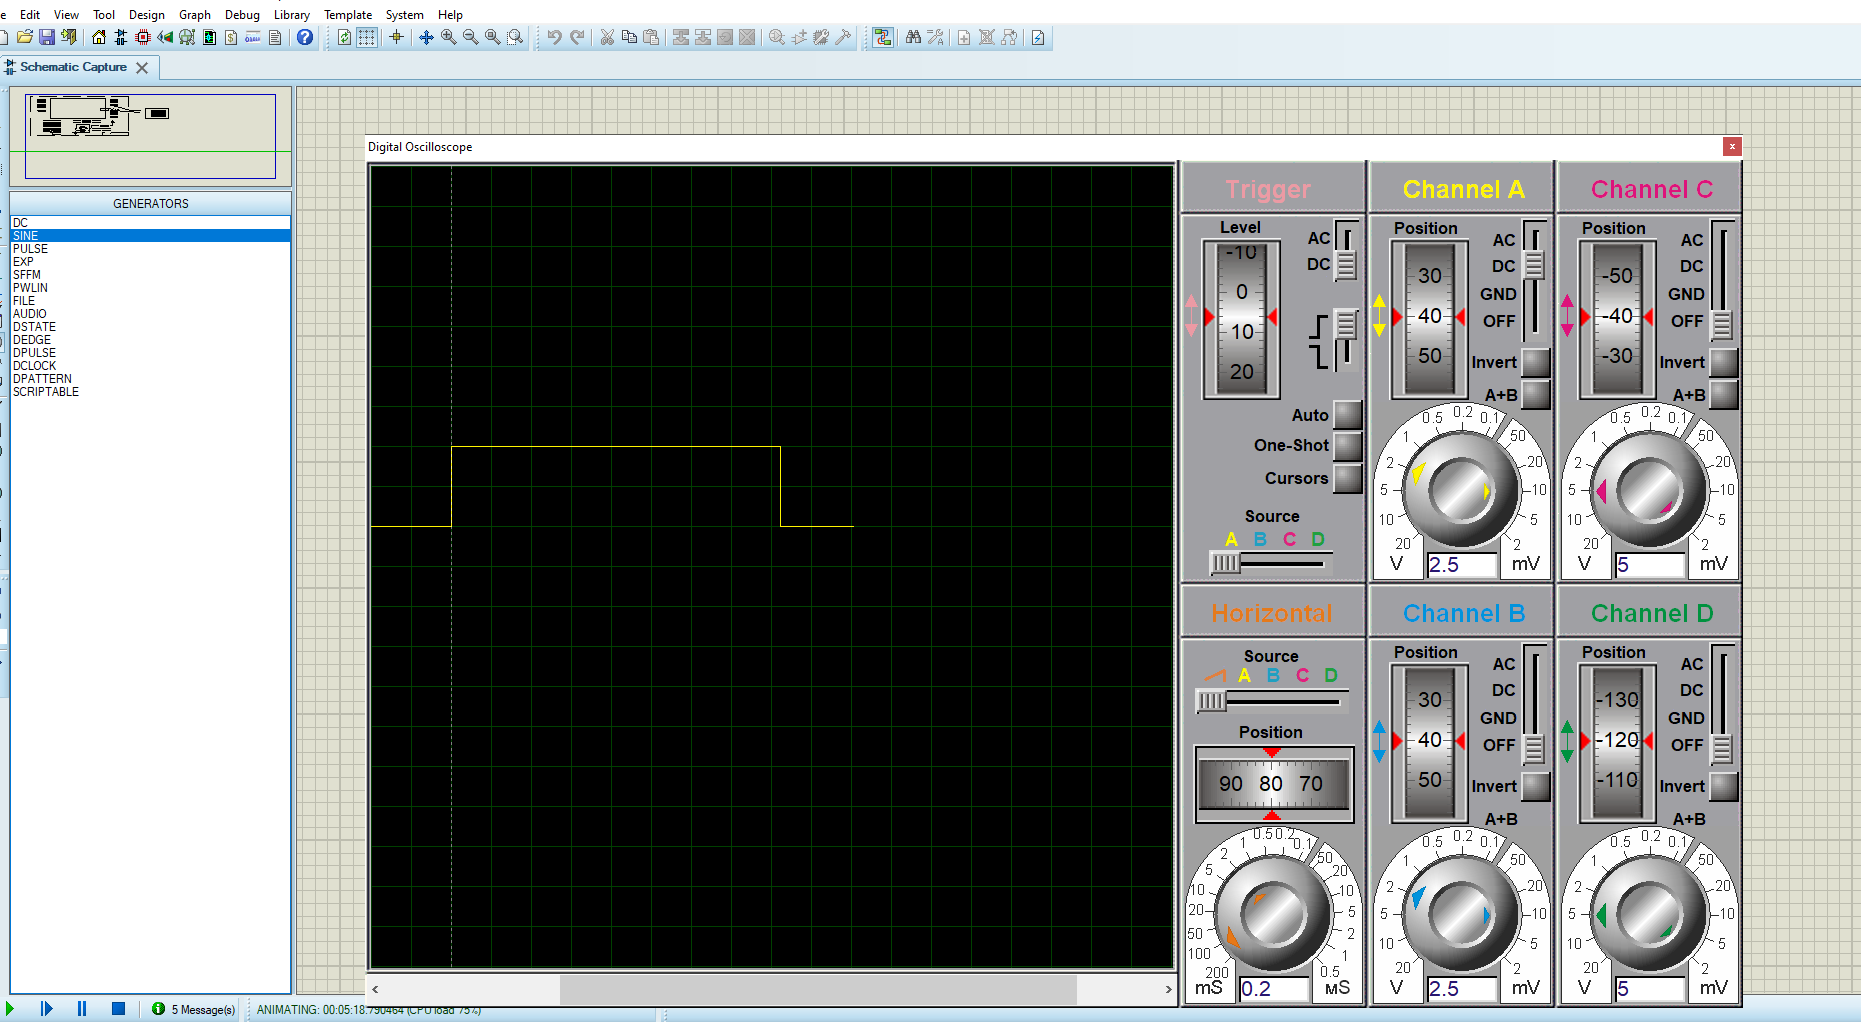
\includegraphics[width=0.43\textwidth]{./proteus_captura.png}
  \caption{Captura de la medición en Proteus}
  \label{fig:proteus_captura}
\end{figure}

\begin{figure}[H]
  \centering
  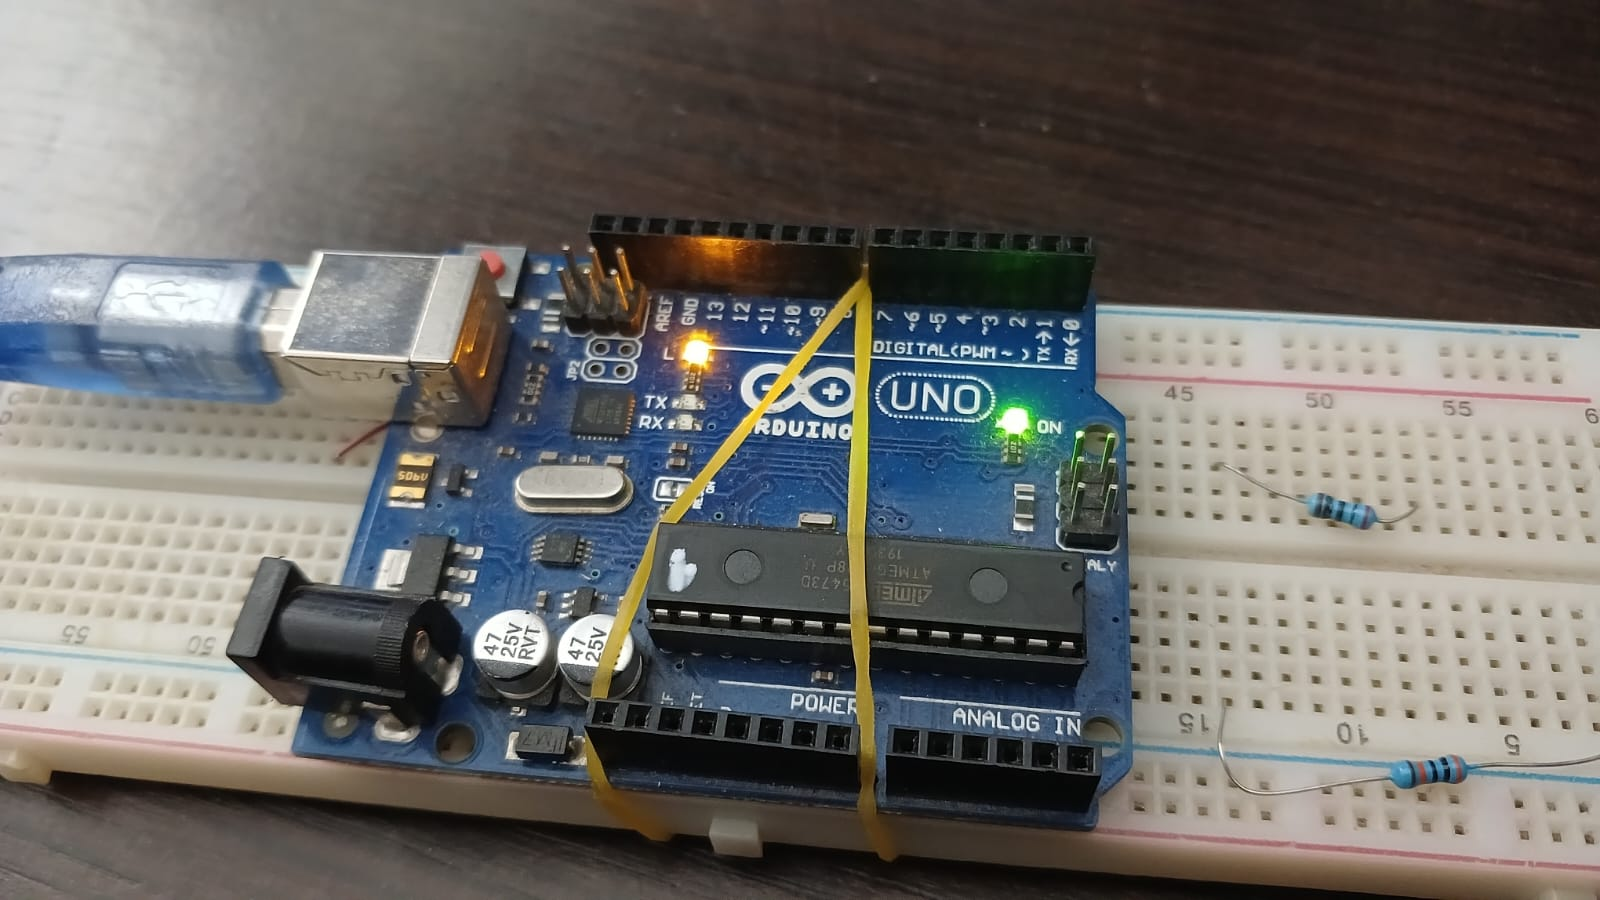
\includegraphics[width=0.43\textwidth]{./placa_real.jpeg}
  \caption{Placa de desarrollo ejecutando el algoritmo}
  \label{fig:placa_real}
\end{figure}

\section{Comparaciones AVR y MARIE}
Para ver el rendimiento de la implementación en AVR, en comparación con la de MARIE, en el debuger de Microchip Studio se calculó cuantos ciclos de reloj le lleva al AVR concretar el ordenamiento, para el mejor y el peor de los casos de ordenamiento (y también el promedio entre ambos), aunque Bubble Sort tiene un coste aproximadamente constante, por lo que deberían ser resultados similares (cosa que ocurre como se puede apreciar en la tabla de resultados \ref{tab:cant_instrucciones}). Una vez que se tienen las instrucciones de ambas arquitecturas se pueden calcular los ciclos de reloj sabiendo que de media MARIE ejecuta una instrucción cada 7 ciclos de reloj, por lo tanto: $CPI_{MARIE} \cong 7$, entonces se puden aproximar los ciclos de reloj haciendo $instrucciones CPI \cong ciclos$; haciendo el mismo análisis para AVR se tiene que $CPI_{AVR} \cong 1.5$ (los resultados de los cálculos se pueden apreciar en la tabla \ref{tab:cant_instrucciones}).

\begin{table}[H]
  \centering
  \begin{tabular}{|l|l|l|}
    \hline
                  & Cantidad de                       & Cantidad de               \\ 
                  & Instrucciones                     & Ciclos de reloj           \\ 
                  &               (mín/media/máx)     & (mín/media/máx)           \\ \hline
    AVR           & 918 / 939 / 960                   & 1377 / 1409 / 1440        \\ \hline
    MARIE         & 534 / 566 / 597                   & 3738 / 3962 / 4179        \\ \hline
  \end{tabular}
  \caption{Instrucciones y ciclos de reloj en AVR y MARIE}
  \label{tab:cant_instrucciones}
\end{table}

\begin{table}[H]
  \centering
  \begin{tabular}{|l|l|l|}
    \hline
                      & Cantidad de instrucciones   & Porcentaje sobre el total   \\ \hline
    Memoria programa  & 160                         & 0.5\%                       \\ \hline
    Memoria datos     & 256                         & 12.5\%                      \\ \hline
  \end{tabular}
  \caption{Espacio que ocupa el programa según Microchip Studio}
  \label{tab:memorio_resultado}
\end{table}

Teniendo presente los calculos previos se puede calcular la mejora que tiene AVR sobre MARIE aplicando las siguientes ecuaciónes
\begin{equation*}
  t = \frac{N*CPI}{f_{reloj}}
\end{equation*}
Considerando un reloj de 16Mhz (aunque es indiferente para el Speedup)
\begin{equation*}
  t_{AVR} \cong 88\mu segundos
\end{equation*}
\begin{equation*}
  t_{MARIE} \cong 248\mu segundos
\end{equation*}
\begin{equation*}
  S (speedup) = \frac{t_{MARIE}}{t_{AVR}} \cong 2.8
\end{equation*}

Por lo que se concluye que la implementación en AVR es 2.8 veces mejor que la de MARIE.

\end{document}
